\chapter{User Guide} % Chapter 2
%

%\nocite{*}

\section{Introduction} % a.
This chapter covers all that is required from the users computer when running the AHED system. The AHED system has an interface for user interaction and provides live feedback on facial expressions. The interface is simple, see Figure~\ref{fig:gui}, and has the following funtionalities:
\begin{itemize}
\item A live video output stream. 
\item Real time emotion classification on the right hand side of the screen. This is where each emotion probability is given for the frame.
\item An Emoji(icon) that dispays the dominant emotion in the frame.
\item `Start Video' Button -- Initiates the video output stream.
\item `End Video' Button -- Pauses the video output stream.
\item `Quit' Button -- Closes the program window.
\end{itemize}
\begin{figure}[H]
  \centering
  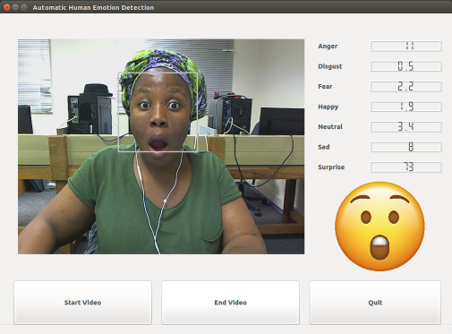
\includegraphics[scale= 0.8]{gui}
  \caption{The Graphical User Interface for the AHED System}
  \label{fig:gui}
\end{figure} 


\subsection{System Requirements}
These are the packages and programs needed to run the AHED system:
\begin{itemize}
\item Python 2.7
\item PyQt4
\item OpenCV
\item Webcamera (preferably HD 1080p)
\item Scikit-Image
\item Numpy
\item Pickle
\item Windows 10 or Ubuntu 16.04 operating sytem (preferably x64 and needs to support the libraries and packages above)
\item Note: Use JetBrains PyCharm on Windows, makes it easier to install missing libraries from python.
\end{itemize}

\subsection{Instructions}
Download `AHED.zip' from `http://cs.uwc.ac.za/~tlehata/index.html' under `Term 4'. After ensuring that your system requirements meet those stated above, unzip the `AHED.zip' folder. Open a terminal window or CMD window in the folder that contains `guiAHED.py'. To continue follow the instructions under your desired operating system.
\subsubsection{Ubuntu}
\begin{itemize} 
\item \$ workon cv
\item \$(cv) python guiAHED.py 
\end{itemize}
\subsubsection{Ubuntu}
\begin{itemize}
\item \$ python guiAHED.py 
\end{itemize}
A window should open up after a few seconds that looks the same as the one in Figure~\ref{fig:start}. After that you can proceed and press `Start Video' to start interacting with the system.
\begin{figure}[H]
  \centering
  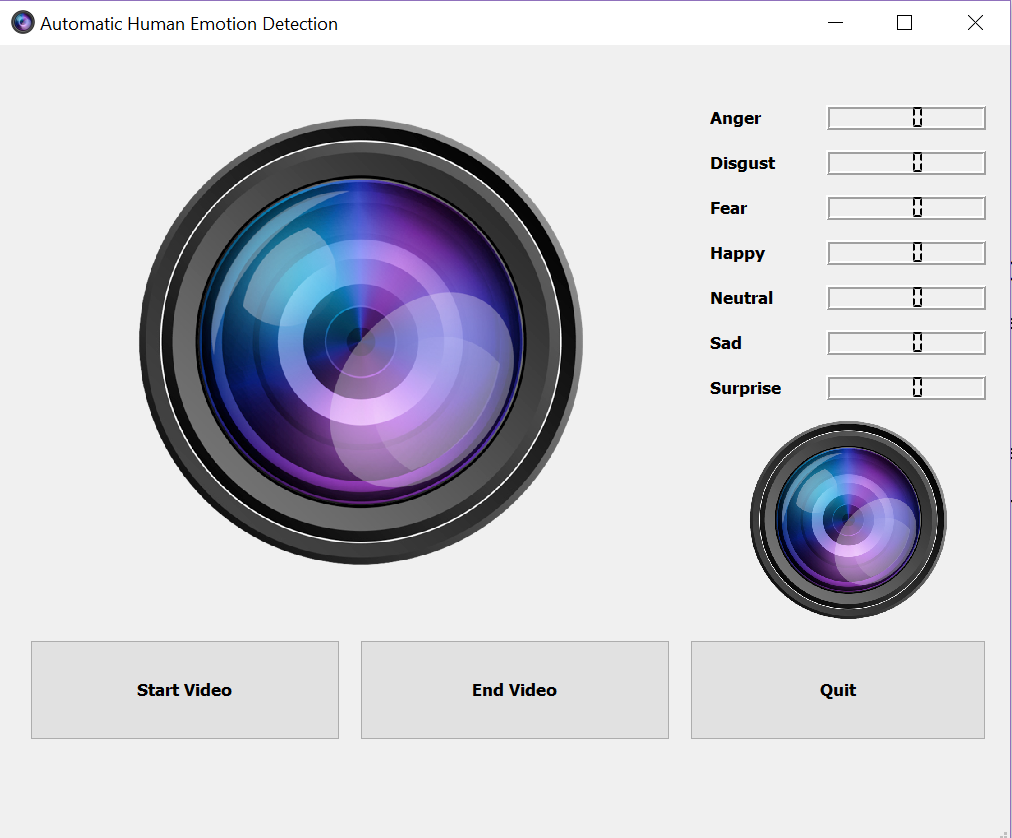
\includegraphics[scale=0.5]{start}
  \caption{Initial Start Interface for the AHED System}
  \label{fig:start}
\end{figure} 

\subsection{Feedback}
To leave feedback or for further assistance and questions send me an email on `3342317@myuwc.ac.za'.